\documentclass[11pt]{article}
\usepackage{amsmath,amssymb,amsthm}
\usepackage{geometry}
\usepackage{booktabs}
\usepackage{graphicx}
\usepackage{hyperref}
\usepackage{enumerate}
\usepackage{listings}
\usepackage{xcolor}
\usepackage{fancyhdr}
\usepackage{tikz}
\usetikzlibrary{arrows.meta,positioning,shapes.geometric}

\geometry{letterpaper, margin=1in}

\lstset{
  basicstyle=\ttfamily\small,
  breaklines=true,
  columns=fullflexible,
  keepspaces=true,
  language=C++,
  keywordstyle=\color{blue}\bfseries,
  commentstyle=\color{gray},
  stringstyle=\color{red!60!black}
}

\pagestyle{fancy}
\fancyhf{}
\fancyhead[L]{\small Emergence Dataset \#1}
\fancyhead[R]{\small VSEPR-SIM}
\fancyfoot[C]{\thepage}

\title{\textbf{Emergence Dataset \#1:} \\
\Large Anisotropy, Isomer Stability, and Fall Transitions}
\author{VSEPR-SIM Development}
\date{Version 1.0.0}

\begin{document}
\maketitle

\begin{abstract}
Emergence Dataset \#1: Anisotropy and Isomer-Fall Transitions is a structured
benchmark for directional-response and state-transition phenomena across
molecular, cluster, and coarse-grained systems. The dataset records initial
and final structural states, anisotropy descriptors, driving perturbations,
transition barriers, persistence times, and fall-event classifications.
Its purpose is to support deterministic simulation studies of symmetry breaking,
metastability, conformational switching, field-induced transitions, and
anisotropy-driven collapse events within the VSEPR-SIM architecture.
\end{abstract}

\tableofcontents
\newpage

% ====================================================================
\section{Core Scientific Idea}
% ====================================================================

The dataset captures two coupled behaviours:

\subsection{Anisotropy}

A system has direction-dependent behaviour. This can be mechanical, electrical,
optical, geometric, transport-related, or energetic. Anisotropy is a standard
property class in materials science and molecular systems.

\subsection{Isomer Fall}

\begin{quote}
\textbf{Isomer Fall} := a discrete transition from one local structural state
to another under perturbation.
\end{quote}

That perturbation may be thermal, field-driven, flow-driven, collision-driven,
stress-driven, radiation-driven, or concentration-driven.

The dataset backbone is:
\begin{equation}
\boxed{\text{State} \;\to\; \text{Perturbation} \;\to\; \text{Directional Response} \;\to\; \text{Structural Transition}}
\end{equation}

% ====================================================================
\section{Dataset Organisation}
% ====================================================================

\begin{center}
\begin{tabular}{clp{8cm}}
\toprule
\textbf{Subset} & \textbf{Name} & \textbf{Scope} \\
\midrule
ED1A & Molecular & Small molecules, torsions, ring flips, cis/trans \\
ED1B & Coordination & Metal centres, ligand distortions, actinide assemblies \\
ED1C & Bead/Structure & Directional collapse, branch reorientation, field-driven deformation \\
\bottomrule
\end{tabular}
\end{center}

This prevents butane and plutonium-ligand bead assemblies from occupying the same row.

% ====================================================================
\section{Isomer-Fall Detection Criteria}
% ====================================================================

A sample is tagged as an isomer-fall event if \textit{any} of the following
conditions hold:

\begin{align}
\Delta E_{\text{barrier}} &< E_{\text{perturb}} \label{eq:barrier} \\
\text{RMSD}(X_t, X_{\text{ref}}) &> \tau_{\text{geom}} \label{eq:rmsd} \\
q_{\text{state}}(t + \Delta t) &\neq q_{\text{state}}(t) \label{eq:label}
\end{align}

where:
\begin{itemize}
  \item $\Delta E_{\text{barrier}}$ = barrier to alternate configuration
  \item $E_{\text{perturb}}$ = supplied perturbation energy
  \item $\text{RMSD}$ = structural displacement (root-mean-square deviation)
  \item $\tau_{\text{geom}}$ = geometric displacement threshold (\AA)
  \item $q_{\text{state}}$ = discrete isomer/state label
\end{itemize}

A fall is not just motion. It is a \textbf{state transition}.

\subsection{Implementation}

\begin{lstlisting}[caption={Fall detection in C++ (emergence\_dataset.hpp)}]
struct FallDetectionConfig {
    double rmsd_threshold{0.5};       // tau_geom (A)
    double barrier_ratio_min{1.0};    // threshold for barrier criterion
    bool   check_state_label{true};   // check q_state change?
};
\end{lstlisting}

% ====================================================================
\section{Anisotropy Descriptors}
% ====================================================================

Anisotropy is not a vibe. It is a quantified ratio.

\subsection{Geometric Anisotropy}

From principal eigenvalues of the gyration tensor:
\begin{equation}
A_{\text{geom}} = \frac{\lambda_1}{\lambda_3}, \quad \lambda_1 \geq \lambda_2 \geq \lambda_3
\end{equation}

Asphericity:
\begin{equation}
\kappa = 1 - \frac{3(\lambda_1 \lambda_2 + \lambda_2 \lambda_3 + \lambda_3 \lambda_1)}{(\lambda_1 + \lambda_2 + \lambda_3)^2}
\end{equation}

\subsection{Mechanical Anisotropy}

\begin{equation}
A_{\text{mech}} = \frac{P_{\max}}{P_{\min}}
\end{equation}

for some property $P$ (modulus, yield response, or compliance).

\subsection{Transport Anisotropy}

\begin{equation}
A_{\text{trans}} = \frac{D_{\parallel}}{D_{\perp}} \quad \text{or} \quad A_{\sigma} = \frac{\sigma_{\parallel}}{\sigma_{\perp}}
\end{equation}

\subsection{Field Anisotropy}

\begin{equation}
A_{E} = \frac{E_{\max, \parallel}}{E_{\max, \perp}}
\end{equation}

\subsection{Optical/Tensor Anisotropy}

\begin{equation}
A_{n} = \frac{n_{\parallel}}{n_{\perp}}
\end{equation}

All ratios are $\geq 1.0$ for anisotropic systems. A ratio of 1.0 means perfectly isotropic.

% ====================================================================
\section{Fall Modes}
% ====================================================================

Categorical labels for the transition type:

\begin{center}
\begin{tabular}{lp{8cm}}
\toprule
\textbf{Mode} & \textbf{Description} \\
\midrule
\texttt{rotation\_fall} & Rigid-body reorientation \\
\texttt{torsion\_fall} & Dihedral angle transition (e.g. anti $\to$ gauche) \\
\texttt{coordination\_fall} & Change in coordination number or shell geometry \\
\texttt{buckling\_fall} & Structural buckling under load \\
\texttt{collapse\_fall} & Compaction / directional collapse \\
\texttt{ligand\_swap\_fall} & Exchange of ligand positions \\
\texttt{electrostatic\_reorientation} & Field-driven dipole realignment \\
\texttt{thermal\_isomerization} & Heat-driven isomer switching \\
\texttt{field\_induced\_isomerization} & External field forces state change \\
\texttt{surface\_binding\_fall} & Adsorption-driven reconfiguration \\
\texttt{conformer\_fall} & Ring flip, chair/boat, etc. \\
\texttt{structural\_fall} & General structural rearrangement \\
\texttt{orientation\_fall} & Facet or axis reorientation \\
\bottomrule
\end{tabular}
\end{center}

% ====================================================================
\section{Fall Severity Score}
% ====================================================================

\begin{equation}
S_f = w_1 \frac{\text{RMSD}}{\text{RMSD}_{\max}} + w_2 \frac{|\Delta E|}{|\Delta E|_{\max}} + w_3 \frac{\tau_{\text{persist}}}{\tau_{\max}}
\end{equation}

where $S_f \in [0, 1]$ and the default weights are:
\begin{center}
\begin{tabular}{ccc}
\toprule
$w_1$ & $w_2$ & $w_3$ \\
\midrule
0.4 & 0.4 & 0.2 \\
\bottomrule
\end{tabular}
\end{center}

Normalisation constants: $\text{RMSD}_{\max} = 5.0$ \AA, $|\Delta E|_{\max} = 50.0$ kcal/mol, $\tau_{\max} = 1000$ ps.

% ====================================================================
\section{Dataset Schema}
% ====================================================================

\subsection{Minimal Schema}

\begin{equation}
X_i = (\text{id}, \; \text{class}, \; C, \; s_0, \; s_1, \; \vec{A}, \; d, \; |d|, \; \tau, \; \Delta E, \; \Delta G, \; \text{RMSD}, \; f, \; m)
\end{equation}

\subsection{Full CSV Header}

\begin{lstlisting}[basicstyle=\ttfamily\scriptsize]
sample_id,family,system_class,composition,charge_state,mass,
initial_state,final_state,transition_class,
anisotropy_type,anisotropy_ratio,
axis_1_x,axis_1_y,axis_1_z,axis_2_x,axis_2_y,axis_2_z,
driver_type,driver_magnitude,temperature_K,pressure_atm,medium,
barrier_energy_kcal,deltaE_kcal,deltaG_kcal,rmsd_A,
residence_time_init_ps,residence_time_final_ps,
fall_flag,fall_mode,fall_severity,
recoverable,hysteresis,metastable,notes
\end{lstlisting}

\subsection{Recommended File Split}

For larger datasets, split into:
\begin{itemize}
  \item \texttt{state.csv} --- identity, states, labels
  \item \texttt{event.csv} --- fall flags, modes, severity
  \item \texttt{tensor.csv} --- anisotropy eigenvalues, axes, ratios
  \item \texttt{environment.csv} --- drivers, T, P, medium
\end{itemize}

% ====================================================================
\section{Label System}
% ====================================================================

\subsection{Binary Labels}

\begin{center}
\begin{tabular}{lp{8cm}}
\toprule
\textbf{Label} & \textbf{Meaning} \\
\midrule
\texttt{fall\_flag} & 0/1 --- did an isomer fall occur? \\
\texttt{recoverable\_flag} & 0/1 --- can the system return to initial state? \\
\texttt{metastable\_flag} & 0/1 --- was the initial state metastable? \\
\bottomrule
\end{tabular}
\end{center}

\subsection{Multiclass Labels}

\texttt{anisotropy\_type}, \texttt{fall\_mode}, \texttt{driver\_type}

\subsection{Continuous Labels}

Anisotropy ratios, barrier energy, RMSD, persistence time, directional tensor eigenvalues.

This provides both supervised ML labels and physically interpretable descriptors.

% ====================================================================
\section{Benchmark Exemplars}
% ====================================================================

\subsection{Example 1: Butane (anti $\to$ gauche)}

\begin{center}
\begin{tabular}{lp{9cm}}
\toprule
\textbf{Field} & \textbf{Value} \\
\midrule
Family & ED1A-Molecular \\
Composition & C$_4$H$_{10}$ \\
Initial state & anti \\
Final state & gauche \\
Trigger & thermal \\
Barrier & 3.4 kcal/mol \\
$\Delta E$ & 0.9 kcal/mol \\
RMSD & 0.8 \AA \\
Fall mode & \texttt{torsion\_fall} \\
Recoverable & yes \\
\bottomrule
\end{tabular}
\end{center}

\subsection{Example 2: Cyclohexane (chair $\to$ boat)}

\begin{center}
\begin{tabular}{lp{9cm}}
\toprule
\textbf{Field} & \textbf{Value} \\
\midrule
Family & ED1A-Molecular \\
Composition & C$_6$H$_{12}$ \\
Initial state & chair \\
Final state & boat \\
Barrier & 10.8 kcal/mol \\
$\Delta E$ & 5.5 kcal/mol \\
Fall mode & \texttt{conformer\_fall} \\
Metastable & yes (boat is metastable) \\
\bottomrule
\end{tabular}
\end{center}

\subsection{Example 3: Organometallic Coordination Shell (trans $\to$ cis)}

\begin{center}
\begin{tabular}{lp{9cm}}
\toprule
\textbf{Field} & \textbf{Value} \\
\midrule
Family & ED1B-Coordination \\
Composition & PtCl$_2$(NH$_3$)$_2$ \\
Initial state & trans (transplatin) \\
Final state & cis (cisplatin) \\
Trigger & electric field \\
Fall mode & \texttt{coordination\_fall} \\
Hysteresis & yes \\
\bottomrule
\end{tabular}
\end{center}

\subsection{Example 4: Anisotropic Crystal Platelet}

\begin{center}
\begin{tabular}{lp{9cm}}
\toprule
\textbf{Field} & \textbf{Value} \\
\midrule
Family & ED1C-Bead/Structure \\
Composition & MoS$_2$ fragment \\
$A_{\text{mech}}$ & 8.5 \\
Trigger & shear stress \\
Fall mode & \texttt{orientation\_fall} \\
Recoverable & yes \\
Hysteresis & yes \\
\bottomrule
\end{tabular}
\end{center}

\subsection{Example 5: Bead-Assembled Structure}

\begin{center}
\begin{tabular}{lp{9cm}}
\toprule
\textbf{Field} & \textbf{Value} \\
\midrule
Family & ED1C-Bead/Structure \\
Composition & CG\_branch\_12bead \\
Initial state & branch\_aligned \\
Final state & collapsed \\
$A_{\text{geom}}$ & 4.2 \\
$\Delta E$ & $-12.0$ kcal/mol \\
Fall mode & \texttt{collapse\_fall} \\
Recoverable & no (irreversible compaction) \\
\bottomrule
\end{tabular}
\end{center}

% ====================================================================
\section{Transition Diagram}
% ====================================================================

\begin{center}
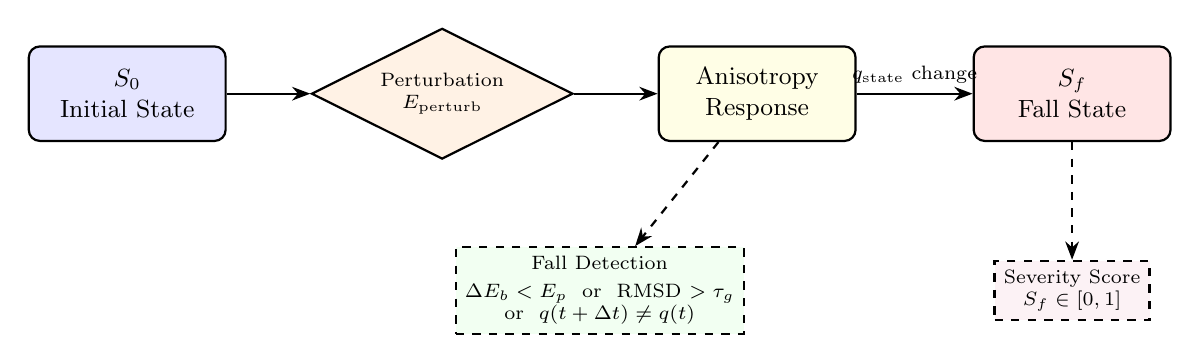
\begin{tikzpicture}[
  state/.style={rectangle, draw, rounded corners, minimum width=2.5cm,
    minimum height=1.2cm, font=\small, align=center},
  driver/.style={diamond, draw, fill=orange!10, aspect=2,
    font=\scriptsize, align=center},
  ->,>=Stealth, thick
]
  \node[state, fill=blue!10] (s0) at (0, 0) {$S_0$\\Initial State};
  \node[driver] (drv) at (4, 0) {Perturbation\\$E_{\text{perturb}}$};
  \node[state, fill=yellow!10] (aniso) at (8, 0) {Anisotropy\\Response};
  \node[state, fill=red!10] (sf) at (12, 0) {$S_f$\\Fall State};

  \draw (s0) -- (drv);
  \draw (drv) -- (aniso);
  \draw (aniso) -- node[above, font=\scriptsize] {$q_{\text{state}}$ change} (sf);

  % Detection criteria
  \node[rectangle, draw, dashed, fill=green!5, font=\scriptsize, align=center]
    (det) at (6, -2.5) {Fall Detection\\[2pt]
    $\Delta E_b < E_p$ ~or~ RMSD $> \tau_g$\\
    or~ $q(t+\Delta t) \neq q(t)$};
  \draw[dashed] (aniso) -- (det);

  % Severity
  \node[rectangle, draw, dashed, fill=purple!5, font=\scriptsize, align=center]
    (sev) at (12, -2.5) {Severity Score\\$S_f \in [0,1]$};
  \draw[dashed] (sf) -- (sev);
\end{tikzpicture}
\end{center}

% ====================================================================
\section{Integration with VSEPR-SIM}
% ====================================================================

\subsection{Mapping to Existing Infrastructure}

\begin{center}
\begin{tabular}{lll}
\toprule
\textbf{ED1 Concept} & \textbf{VSEPR-SIM Component} & \textbf{Header} \\
\midrule
State & \texttt{atomistic::State} / \texttt{StateC} & \texttt{state.hpp} / \texttt{state\_c.hpp} \\
Anisotropy tensor & \texttt{InertiaFrame} & \texttt{inertia\_frame.hpp} \\
RMSD & \texttt{compute\_rmsd()} & \texttt{alignment.hpp} \\
Conformer search & \texttt{ConformerFinder} & \texttt{conformer\_finder.hpp} \\
Fall event & \texttt{EventRecord} in $\Omega$ & \texttt{state\_c.hpp} \\
Provenance & \texttt{SourceTag} ($\Sigma$) & \texttt{state\_c.hpp} \\
Environment & \texttt{Environment} ($\mathcal{E}$) & \texttt{state\_c.hpp} \\
Perturbation & \texttt{PerturbationDriver} & \texttt{emergence\_dataset.hpp} \\
\bottomrule
\end{tabular}
\end{center}

\subsection{Relationship to Dev Day $\sim$42 Notation}

Each emergence sample maps directly to the revised notation:
\begin{itemize}
  \item \textbf{$S_0$}: initial state of the sample (StateC with composition, environment, constraints)
  \item \textbf{$T(S_0, t, \Lambda)$}: perturbation-driven transformation
  \item \textbf{$S_f$}: outcome state after fall (or non-fall)
  \item \textbf{$\Omega$}: event log recording the fall event
  \item \textbf{$Q$}: quality flags indicating whether the fall is trustworthy
\end{itemize}

\subsection{Relationship to Deep Research Engine}

The deep research engine (Phase 10A -- 41A) can feed samples into ED1:
\begin{itemize}
  \item Phase 10A enumerated geometries become ED1A molecular samples
  \item Phase 20B bead formations become ED1C bead/structure samples
  \item SHA-512 pathway hashes provide provenance ($\Sigma$) for each sample
\end{itemize}

% ====================================================================
\section{Project Tree}
% ====================================================================

\begin{lstlisting}[basicstyle=\ttfamily\scriptsize]
atomistic/
  core/
    state.hpp              <-- Particle-level state
    state_c.hpp            <-- Dev Day ~42 revised notation
    alignment.hpp          <-- RMSD, Kabsch alignment
  datasets/
    emergence_dataset.hpp  <-- THIS FILE (ED1 schema + detection + export)
  research/
    deep_research.hpp      <-- 4-phase pipeline (feeds ED1)

coarse_grain/
  core/
    inertia_frame.hpp      <-- Principal-axis decomposition (anisotropy source)
    bead.hpp               <-- Bead struct (C = Bead representation)

src/sim/
  conformer_finder.hpp     <-- Isomer/conformer enumeration

tests/
  test_emergence_dataset.cpp  <-- 25 tests (enums, detection, severity, exemplars)

docs/
  section_emergence_dataset_1.tex  <-- THIS DOCUMENT
\end{lstlisting}

% ====================================================================
\section{Summary}
% ====================================================================

Emergence Dataset \#1 establishes:

\begin{enumerate}
  \item \textbf{Three subfamilies} (ED1A Molecular, ED1B Coordination, ED1C Bead/Structure) preventing forced coexistence of incompatible system types.
  \item \textbf{Strict fall detection} via three independent criteria: barrier energy, RMSD displacement, and state-label change.
  \item \textbf{Quantified anisotropy} through eigenvalue ratios of relevant tensors (geometric, mechanical, transport, field, optical).
  \item \textbf{Categorical fall modes} with a composite severity score $S_f \in [0, 1]$.
  \item \textbf{Five benchmark exemplars} spanning butane torsion, cyclohexane ring flip, transplatin isomerisation, crystal platelet reorientation, and bead-assembly collapse.
  \item \textbf{CSV export} with a full schema header for both single-file and split-file workflows.
  \item \textbf{Direct integration} with the VSEPR-SIM state machine ($S_0 \to T \to S_f$), provenance system ($\Sigma$), event log ($\Omega$), and quality flags ($Q$).
\end{enumerate}

The C++ implementation lives in \texttt{atomistic/datasets/emergence\_dataset.hpp} and is validated by 25 tests covering all schema components, detection logic, anisotropy computation, severity scoring, and benchmark exemplars.

\end{document}
